\documentclass[a4paper, amsfonts, amssymb, amsmath, reprint, showkeys, nofootinbib, twoside]{revtex4-1}
\usepackage[english]{babel}
\usepackage[utf8]{inputenc}
\usepackage[colorinlistoftodos, color=green!40, prependcaption]{todonotes}
\usepackage[pdftex, pdftitle={Article}, pdfauthor={Author}]{hyperref}
\usepackage{amsthm}
\usepackage{mathtools}
\usepackage{physics}
\usepackage{xcolor}
\usepackage{caption}
\usepackage{hyperref}
%\hypersetup{colorlinks=true, linkcolor=blue, urlcolor = blue}
\usepackage{amsmath}
\usepackage{amssymb}
\usepackage{graphicx}
\graphicspath{Images}
\usepackage[left=23mm,right=13mm,top=35mm,columnsep=15pt]{geometry} 
\usepackage{adjustbox}
\usepackage{placeins}
\usepackage[T1]{fontenc}
\usepackage{float}
%\usepackage{longtable}
\usepackage{csquotes}
\usepackage{refstyle}
\usepackage{lipsum}




\begin{document}

\title{Determination of wavelength of light using Michelson's Interferometer}
\author{Swaroop Ramakant Avarsekar}
\email{swaroop.avarsekar@niser.ac.in}
\affiliation{School of Physical Sciences, National Institute of Science Education and Research, HBNI, Jatni -752050, India}
\date{31 August, 2022}


	
\begin{abstract}
Michelson's Interferometer is used to determine the wavelength of the light source by interference. The aim of this experiment is to find the wavelength of He-Ne Laser beam and sodium lamp from Michelson's interferometer by measuring the number of fringes appearing or disappearing as one of the mirror is moved by some distance keeping other mirror at fixed position. Concentric circular fringes, usually called fringes of equal inclination, is obtained when the two mirror of the interferometer are aligned parallel along an axis, else curved fringes, called fringes of equal thickness, are obtained when those mirrors are tilted forming wedge shaped air film. We found that the wavelength of He-Ne laser is 635.56 ± 9.20 nm and wavelength of sodium lamp is 566.98 ± 17.22 nm.
\end{abstract}
	
\keywords{Interference, Fringes, Path difference}
	
\maketitle

\section{Introduction}

Michelson interferometer, devised by Albert Michelson, is an amplitude splitting interferometer which consists of two mirrors placed perpendicular to each other with a beam splitter inclined at $45^{\circ}$ to both mirrors. The beam splitter is semi-silvered which reflects as well as transmits the light, equally. After passing though beam splitter, the light reflects back from the two mirrors back to beam splitter combining the amplitudes by principle of superposition interfere on any plane between to form fringes. A schematic diagram of this interferometer is given in Figure (\ref{mi}). This interferometer was used in Michelson-Morley experiment to detect the existence of ether in space. 

\section{Theory}
\begin{figure}[htbp]
\begin{center}
\includegraphics[width=6.5 cm]{d1}
\caption{A schematic diagram of Michelson's interferometer}
\label{mi}
\end{center}
\end{figure}

From the image above, mirror $M_1$ is movable where virtual image is $M'_2$ of mirror $M_2$ formed in mirror $M_1$. Let d=$x_1-x_2$ be the path difference.
The beam splitter introduces an additional phase shift of $\pi$ for the beam reflected from $M_2$. The condition for the \\constructive interference is
\begin{equation}
2d.cos\theta=\left(n+\frac{1}{2}\right)\lambda
\end{equation}
whereas for the destructive interference is \\
\begin{equation}
2d.cos\theta=n\lambda
\label{e2}
\end{equation}
%\newline
where n=0, 1, 2... \newline
$\lambda$ is wavelength of light used \newline
$\theta$ is angle rays make with the axis of the mirrors (In this case, $\theta$ is $0^{\circ}$)
\newline
\newline
As the d decreases, the fringes begin to collapse at the centre. As the mirror $M_1$ is moved till $x_2=x_1$ we see no fringe at all, and if the d increases then fringes begin to appear. 
\newline
If the one of the mirror is moved by $\Delta d$ and N fringes collapse or appear at the centre then,
\begin{equation}
2(d+\Delta d)=(n+N)\lambda
\label{e3}
\end{equation}

Therefore, from equation (\ref{e2}) and (\ref{e3}), 
\begin{equation}
2\Delta d=N\lambda
\end{equation}

Wavelength of light source,
\begin{equation}
\lambda=\frac{2\Delta d}{N}
\label{f}
\end{equation}

The compensating plate is also used, placed between the mirror $M_2$ and beam splitter with the same angle that of beam splitter, in the apparatus whose purpose is to compensate for the extra optical path $2(\mu-1)t$, where $t$ is thickness and $\mu$ is the refractive index of the beam splitter, by increasing the coherence of light beams. The compensating plate is identical to beam splitter without reflective coating.
Compensating plate is essential in case of producing fringes from white light as it is not possible to get zero path difference for all the wavelengths, since refractive index depends on wavelength.

\begin{figure}[htbp] %  figure placement: here, top, bottom, or page
   \centering
   \includegraphics[width=8.3cm]{fri1} 
   \caption{Fringes of equal inclination}
   \label{}
\end{figure}

\begin{figure}[htbp] %  figure placement: here, top, bottom, or page
   \centering
   \includegraphics[width=8.3cm]{fri2} 
   \caption{Fringes of equal thickness}
   \label{}
\end{figure}

The fringes obtained when two mirrors are perpendicular to each other is called \textbf{fringes of equal inclination}. These are concentric circular fringes. If the distance of these two mirrors are equal from the beam splitter, then no fringes can be seen. If the two mirrors are not perpendicular with each other, by making an angle $\theta$, \textbf{fringes of equal thickness} is obtained, which are usually curved arcs. If the mirror is moved by distance such that  the virtual image $M'_2$ intersects $M_1$, straight line fringes are obtained.

\section{Experiment}
\subsection{Apparatus}
\begin{figure}[htbp] %  figure placement: here, top, bottom, or page
   \centering
   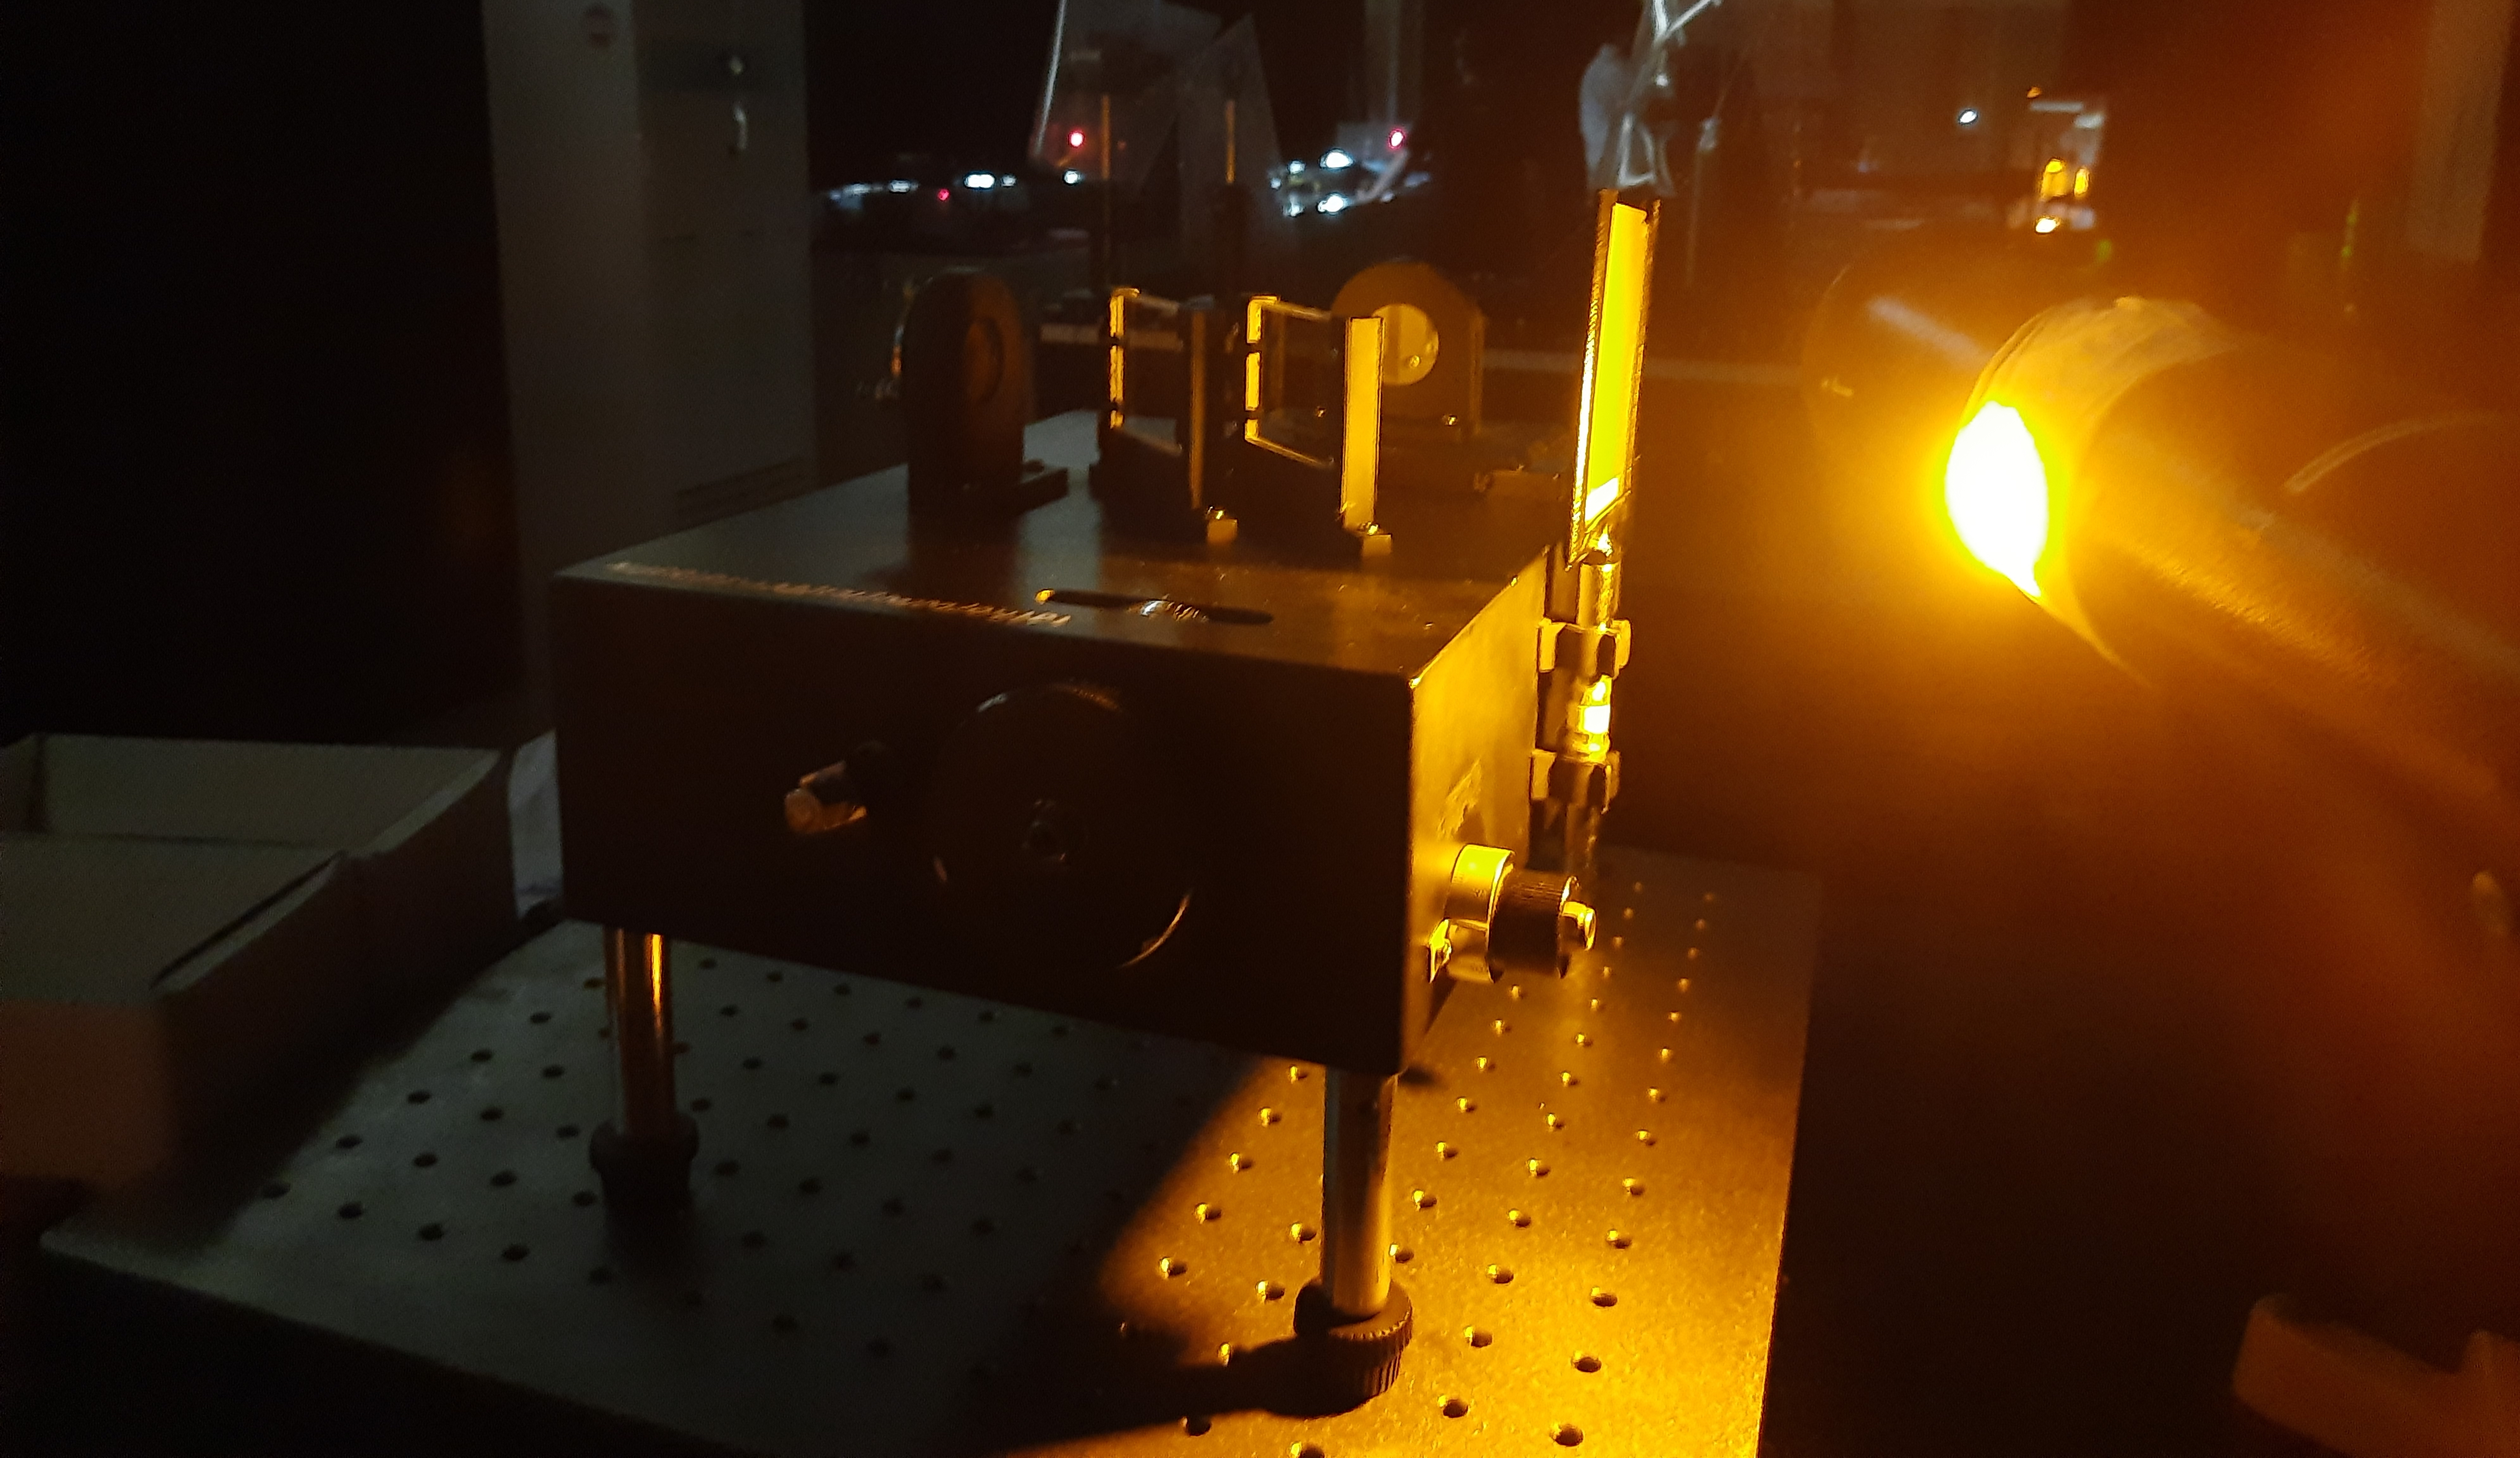
\includegraphics[width=8.3cm]{exp} 
   \caption{Experimental setup with sodium lamp}
   \label{Na}
\end{figure}

\begin{figure}[htbp] %  figure placement: here, top, bottom, or page
   \centering
   \includegraphics[width=8.3cm]{exp1} 
   \caption{Experimental setup with He-Ne laser}
   \label{la}
\end{figure}

The apparatus consists of Michelson's interferometer with He-Ne laser and Sodium lamp as light source. Michelson's interferometer is placed on the optical table with light source placed on the lab jack such that the mirror, beam splitter and the light source are in the same axis. Beam expander will be required when we use laser, it expands the beams to get better view of the fringes. The pin-hole is used to adjust the reflected beams and glass plate to view the fringes, A telescope may also be used to aid the view of the fringes in the case of sodium lamp as light source. A screen is placed at 1-2 metres apart from the apparatus to view the fringes. Experimental apparatus in the lab is as shown in Figure (\ref{Na}) and (\ref{la}).

\subsection{Procedure}
Place the Michelson's interferometer on the optical table, with the coarse adjustment towards your side and adjust the lab jack with the He-Ne laser placed on it such that the laser beam is parallel and strikes the centre of the mirror. The screen should be placed at-least 1m apart from the setup to get better resolution along the axis of movable mirror. Adjust the mirror position by tilting screws seeing the reflected beams on the screen placed, such that reflected beam which is intense should coincide so that interference could take place. The faint beam is also seen due to reflection from un-silvered surface of beam splitter and mirrors. Change the distance of movable mirror such that two mirrors are equidistant from the beam splitter. If two mirrors are exactly perpendicular then it is said to be in normal adjustment provided the condition that beam splitter bisects the two mirrors with $45^{\circ}$. Adjust the position of beam expander along the axis of the laser beam such that the concentric fringes are visible on the screen. 

Move the mirror using fine adjustment knob slowly such that fringes appear or collapse on the screen. Measure the reading of coarse and fine adjustment scale $m$ and $n$ then multiply it by least count 0.01 mm and 0.0001 mm, respectively. Add both to get total reading. Let this be initial reading $d_1$. Count the number of fringes appearing/ collapsing to be N. Note down the reading $d_2$ with the same procedure. Subtract $d_2$ and $d_1$ to get value of $d$. Repeat the process for few observations. For simplicity, we took N to be around 20 fringes. The same procedure can be followed for sodium lamp as well. Here, the intense beams of the sodium lamp should be adjusted by the pinhole and beam expander should be replaced with glass screen. In this case, there is no need of screen as the fringes will be visible with naked eye along the axis of movable mirror. Telescope can be used to aid the viewing. The readings taken must be used in equation (\ref{f}) to determine the wavelength of the He-Ne laser beam and sodium light. 

\subsection{Observations}

\begin{table}[H]
\centering
\caption{For He-Ne Laser source}
\label{mic}
Initial position of the knob, $d_1$=0.3131 mm
\resizebox{\columnwidth}{!}{%
\begin{tabular}{|c |c |c |c |c |c |}
\hline
Sl no &
  \begin{tabular}[c]{@{}c@{}}Number of fringes \\ appearing/disappearing (N)\end{tabular} &
  \begin{tabular}[c]{@{}c@{}}Coarse adjustment \\ reading (m)\end{tabular} &
  \begin{tabular}[c]{@{}c@{}}Fine adjustment \\ count (n)\end{tabular} &
  \begin{tabular}[c]{@{}c@{}}Total reading (mm)\\ $d_2=m\times0.01+n\times0.0001$\end{tabular} &
  \begin{tabular}[c]{@{}c@{}}$\Delta d=d_2-d_1$\\ (mm)\end{tabular} \\ \hline
1  & 20  & 32 & 82 & 0.3282 & 0.0151 \\ \hline
2  & 40  & 33 & 81 & 0.3381 & 0.025  \\ \hline
3  & 60  & 34 & 70 & 0.347  & 0.0339 \\ \hline
4  & 80  & 35 & 48 & 0.3548 & 0.0417 \\ \hline
5  & 100 & 36 & 18 & 0.3618 & 0.0487 \\ \hline
6  & 120 & 36 & 83 & 0.3683 & 0.0552 \\ \hline
7  & 140 & 37 & 44 & 0.3744 & 0.0613 \\ \hline
8  & 160 & 38 & 4  & 0.3804 & 0.0673 \\ \hline
9  & 180 & 38 & 66 & 0.3866 & 0.0735 \\ \hline
10 & 200 & 39 & 26 & 0.3926 & 0.0795 \\ \hline
11 & 220 & 39 & 88 & 0.3988 & 0.0857 \\ \hline
12 & 240 & 40 & 58 & 0.4058 & 0.0927 \\ \hline
13 & 260 & 41 & 12 & 0.4112 & 0.0981 \\ \hline
14 & 280 & 41 & 78 & 0.4178 & 0.1047 \\ \hline
15 & 300 & 42 & 37 & 0.4237 & 0.1106 \\ \hline
16 & 320 & 42 & 95 & 0.4295 & 0.1164 \\ \hline
17 & 340 & 43 & 49 & 0.4349 & 0.1218 \\ \hline
18 & 360 & 44 & 6  & 0.4406 & 0.1275 \\ \hline
19 & 380 & 44 & 58 & 0.4458 & 0.1327 \\ \hline
\end{tabular}%
}
\end{table}

% Please add the following required packages to your document preamble:
% \usepackage{graphicx}
\begin{table}[H]
\centering
\caption{For Sodium Lamp}
\label{nal}
Initial position of the knob, $d_1$=0.0538 mm
\resizebox{\columnwidth}{!}{%
\begin{tabular}{|c|c|c|c|c|c|}
\hline
Sl no &
  \begin{tabular}[c]{@{}c@{}}Number of fringes \\ appearing/disappearing (N)\end{tabular} &
  \begin{tabular}[c]{@{}c@{}}Coarse adjustment \\ reading (m)\end{tabular} &
  \begin{tabular}[c]{@{}c@{}}Fine adjustment\\  count (n)\end{tabular} &
  \begin{tabular}[c]{@{}c@{}}Total reading (mm)\\ $d_2=m\times0.01+n\times0.0001$\end{tabular} &
  \begin{tabular}[c]{@{}c@{}}$\Delta d=d_2-d_1$\\ (mm)\end{tabular} \\ \hline
1 & 20  & 5 & 98 & 0.0598 & 0.006  \\ \hline
2 & 40  & 6 & 43 & 0.0643 & 0.0105 \\ \hline
3 & 60  & 7 & 6  & 0.0706 & 0.0168 \\ \hline
4 & 80  & 7 & 60 & 0.076  & 0.0222 \\ \hline
5 & 100 & 8 & 23 & 0.0823 & 0.0285 \\ \hline
\end{tabular}%
}
\end{table}

\begin{figure}[H] %  figure placement: here, top, bottom, or page
   \centering
   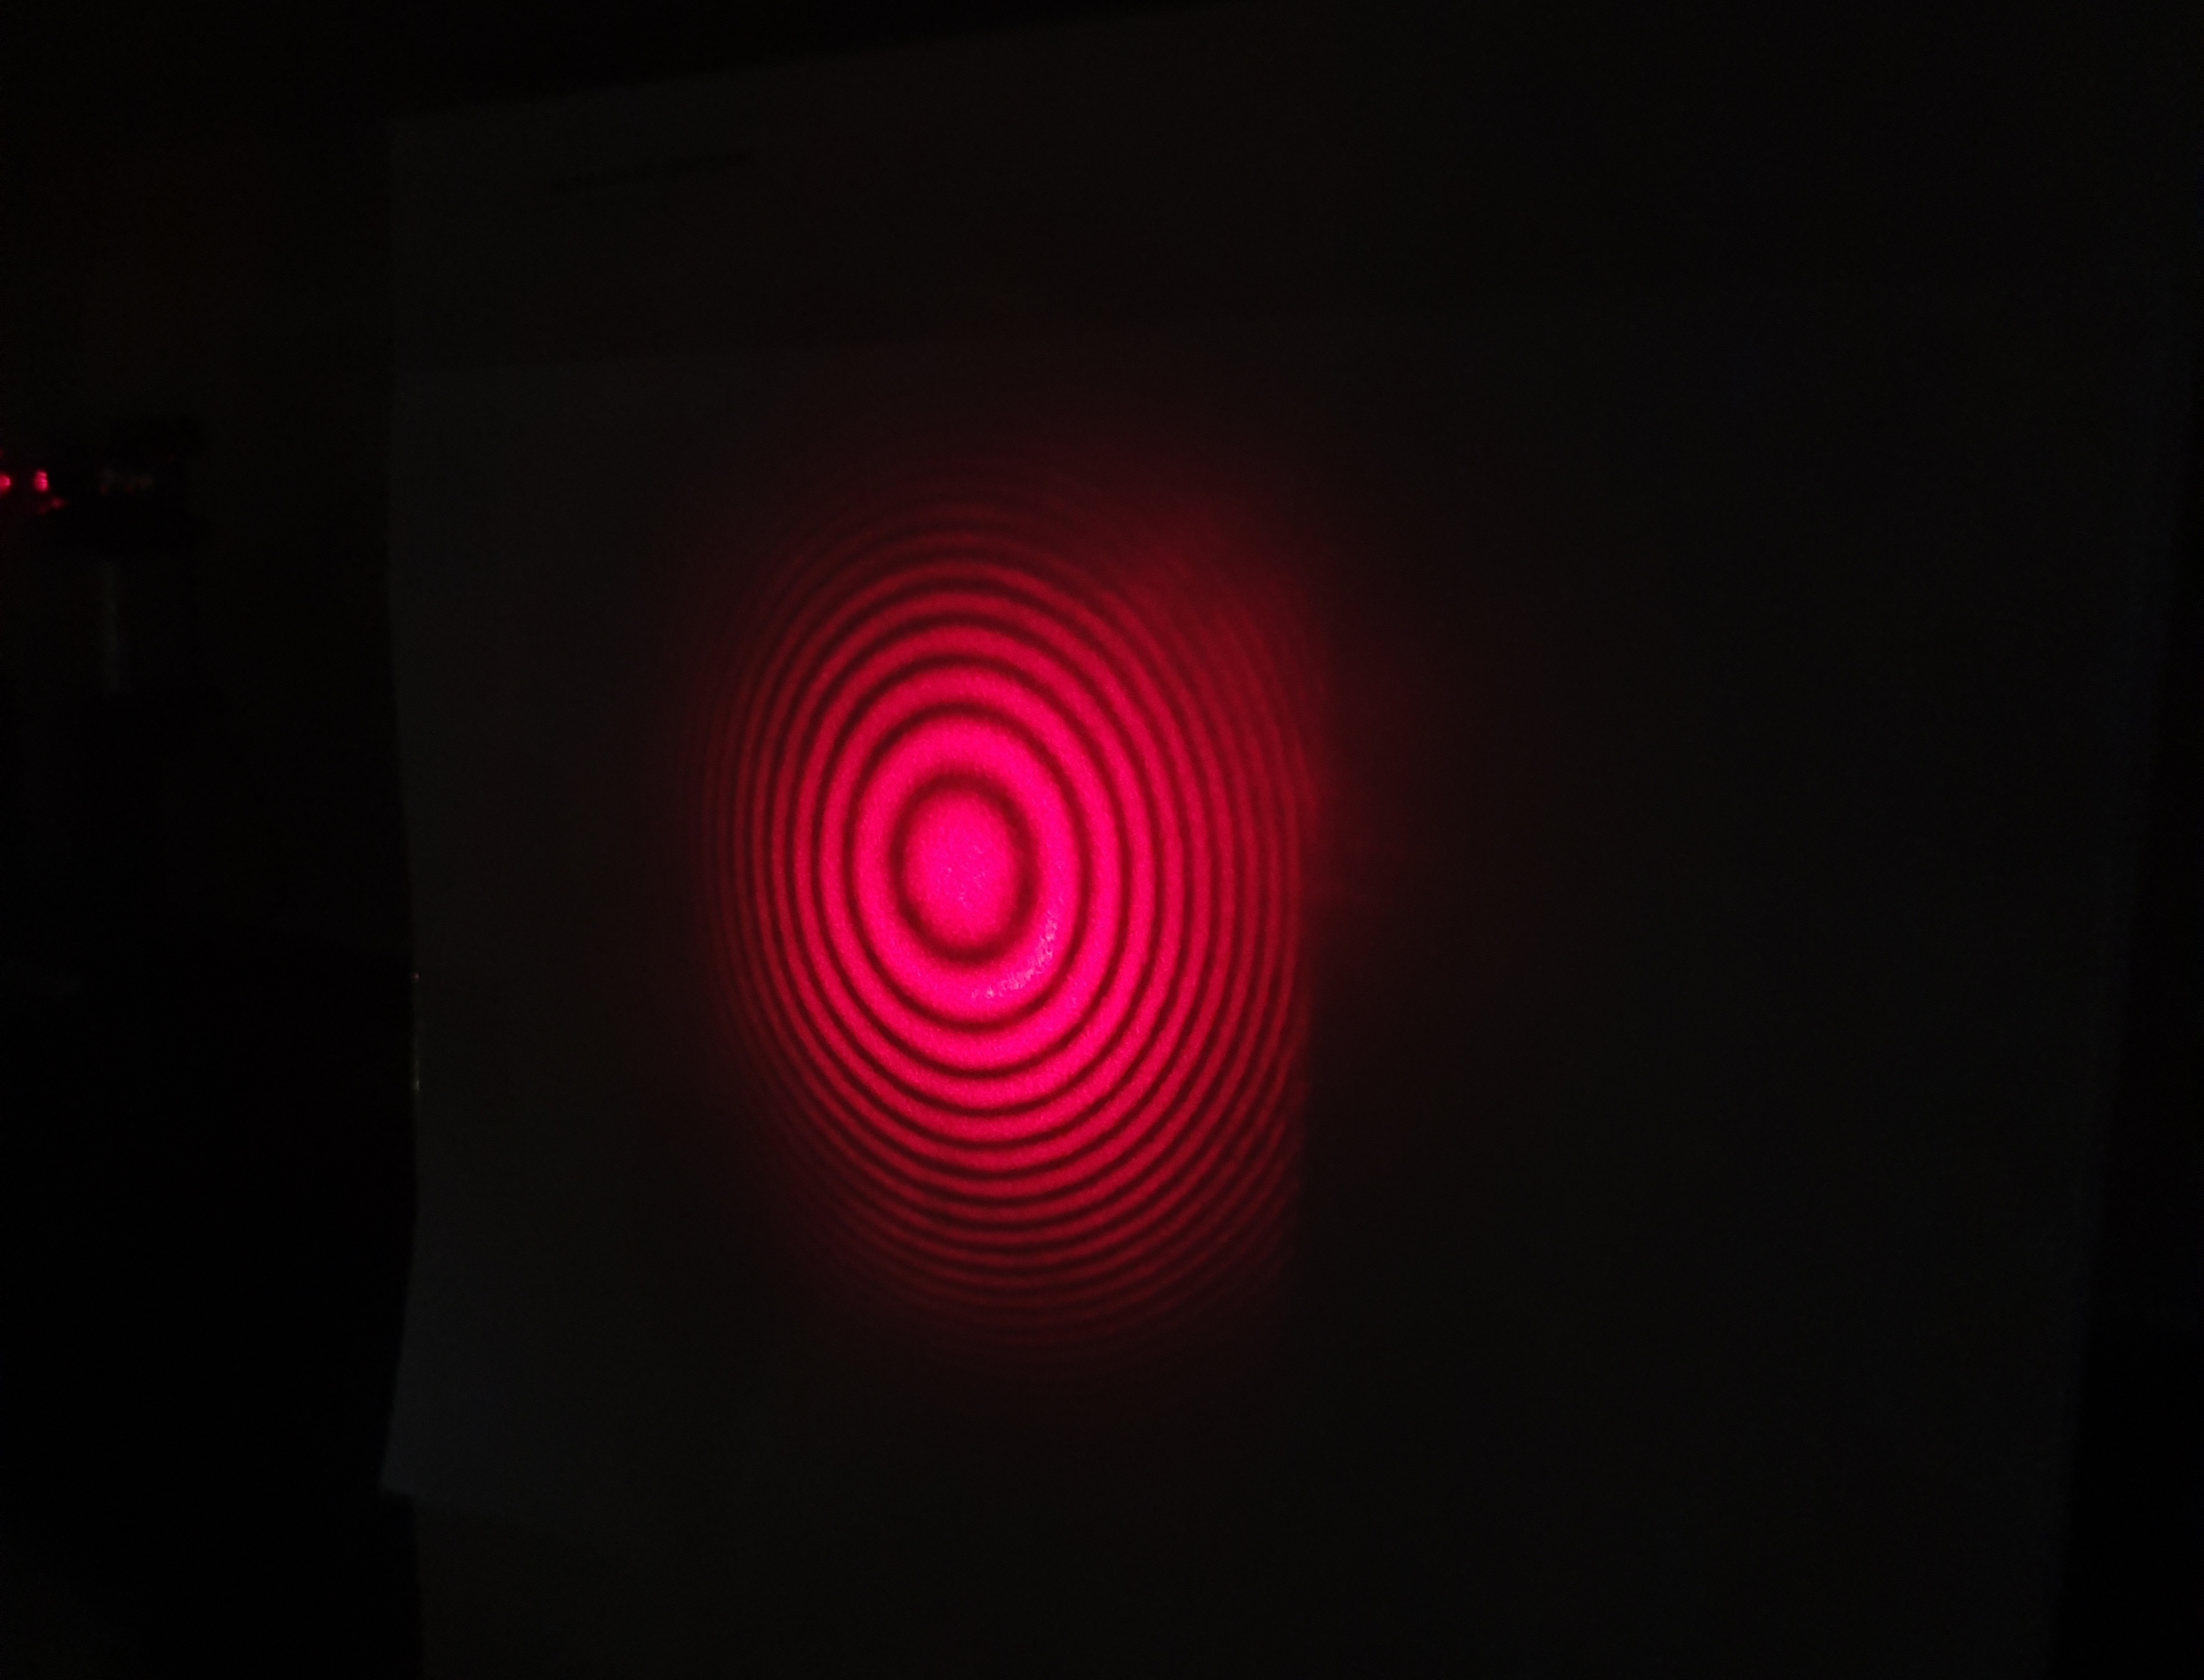
\includegraphics[width=8.3cm]{d3} 
   \caption{Concentric fringes obtained in the case of He-Ne laser as light source}
   \label{redf}
\end{figure}

\begin{figure}%[htbp] %  figure placement: here, top, bottom, or page
   \centering
   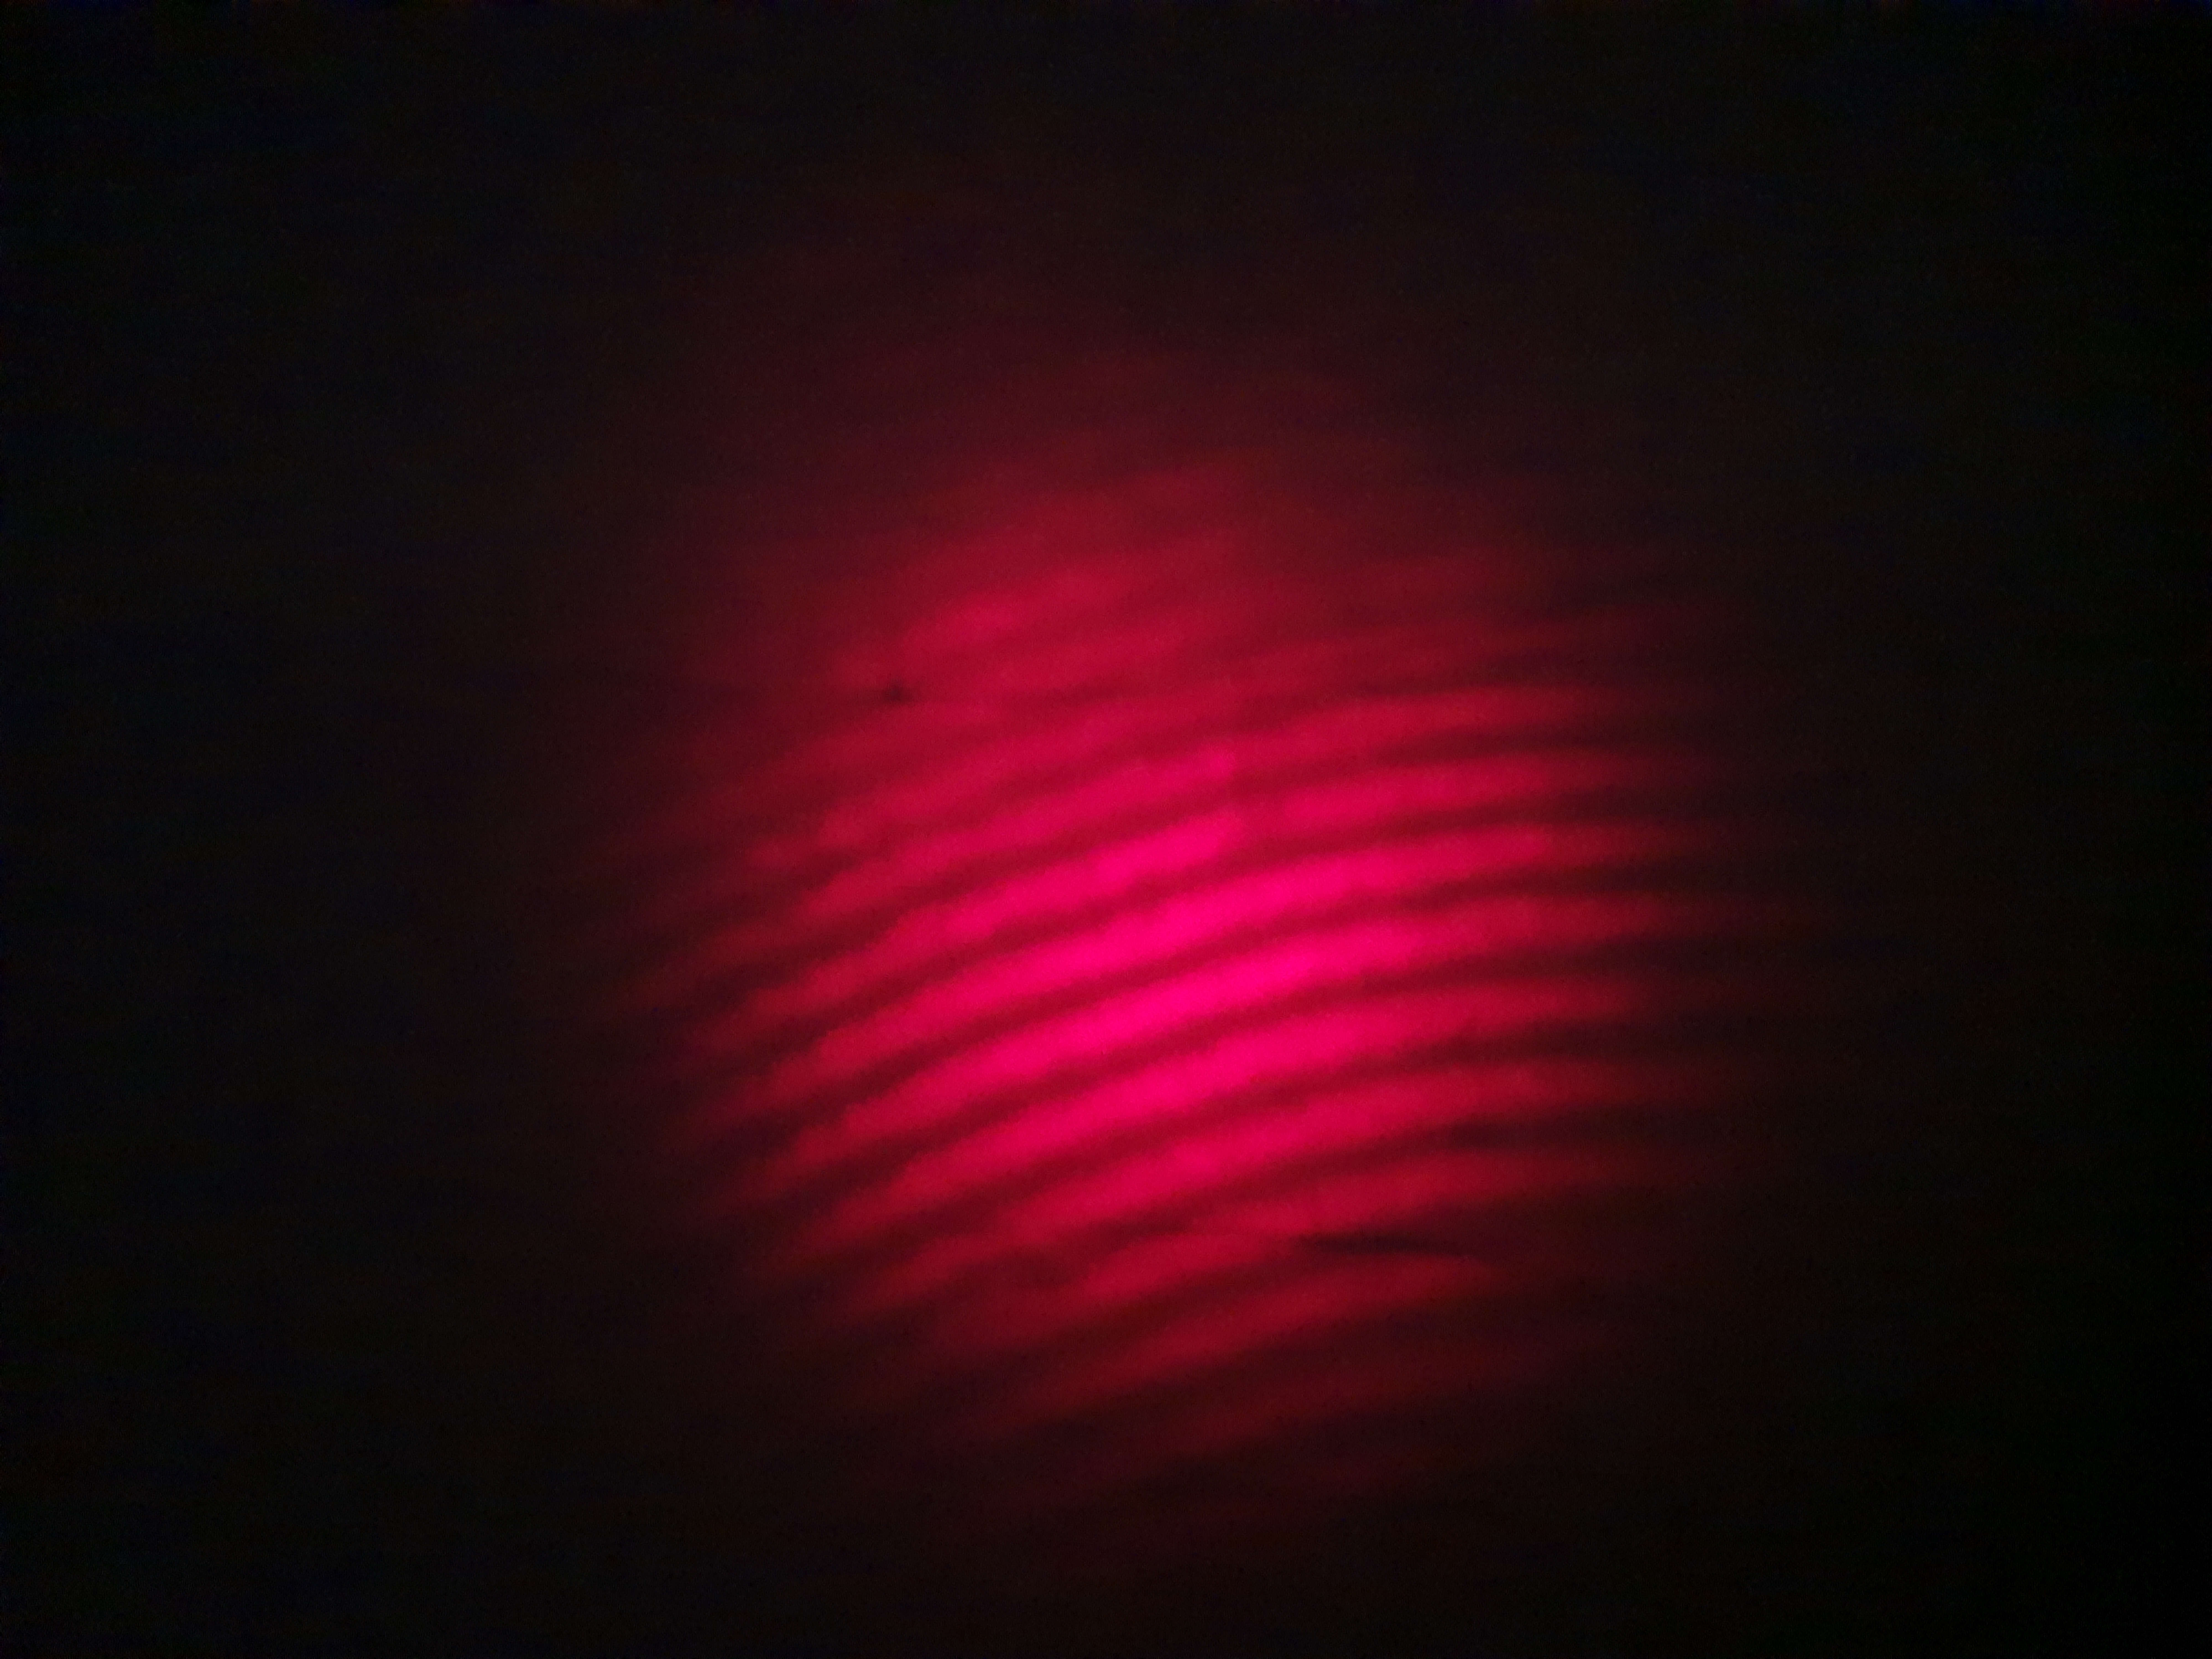
\includegraphics[width=8.3cm]{d2} 
   \caption{Curved fringes when mirrors are tilted by an angle $\theta$ before intersection}
   \label{gd}
\end{figure}

\begin{figure}%[htbp] %  figure placement: here, top, bottom, or page
   \centering
   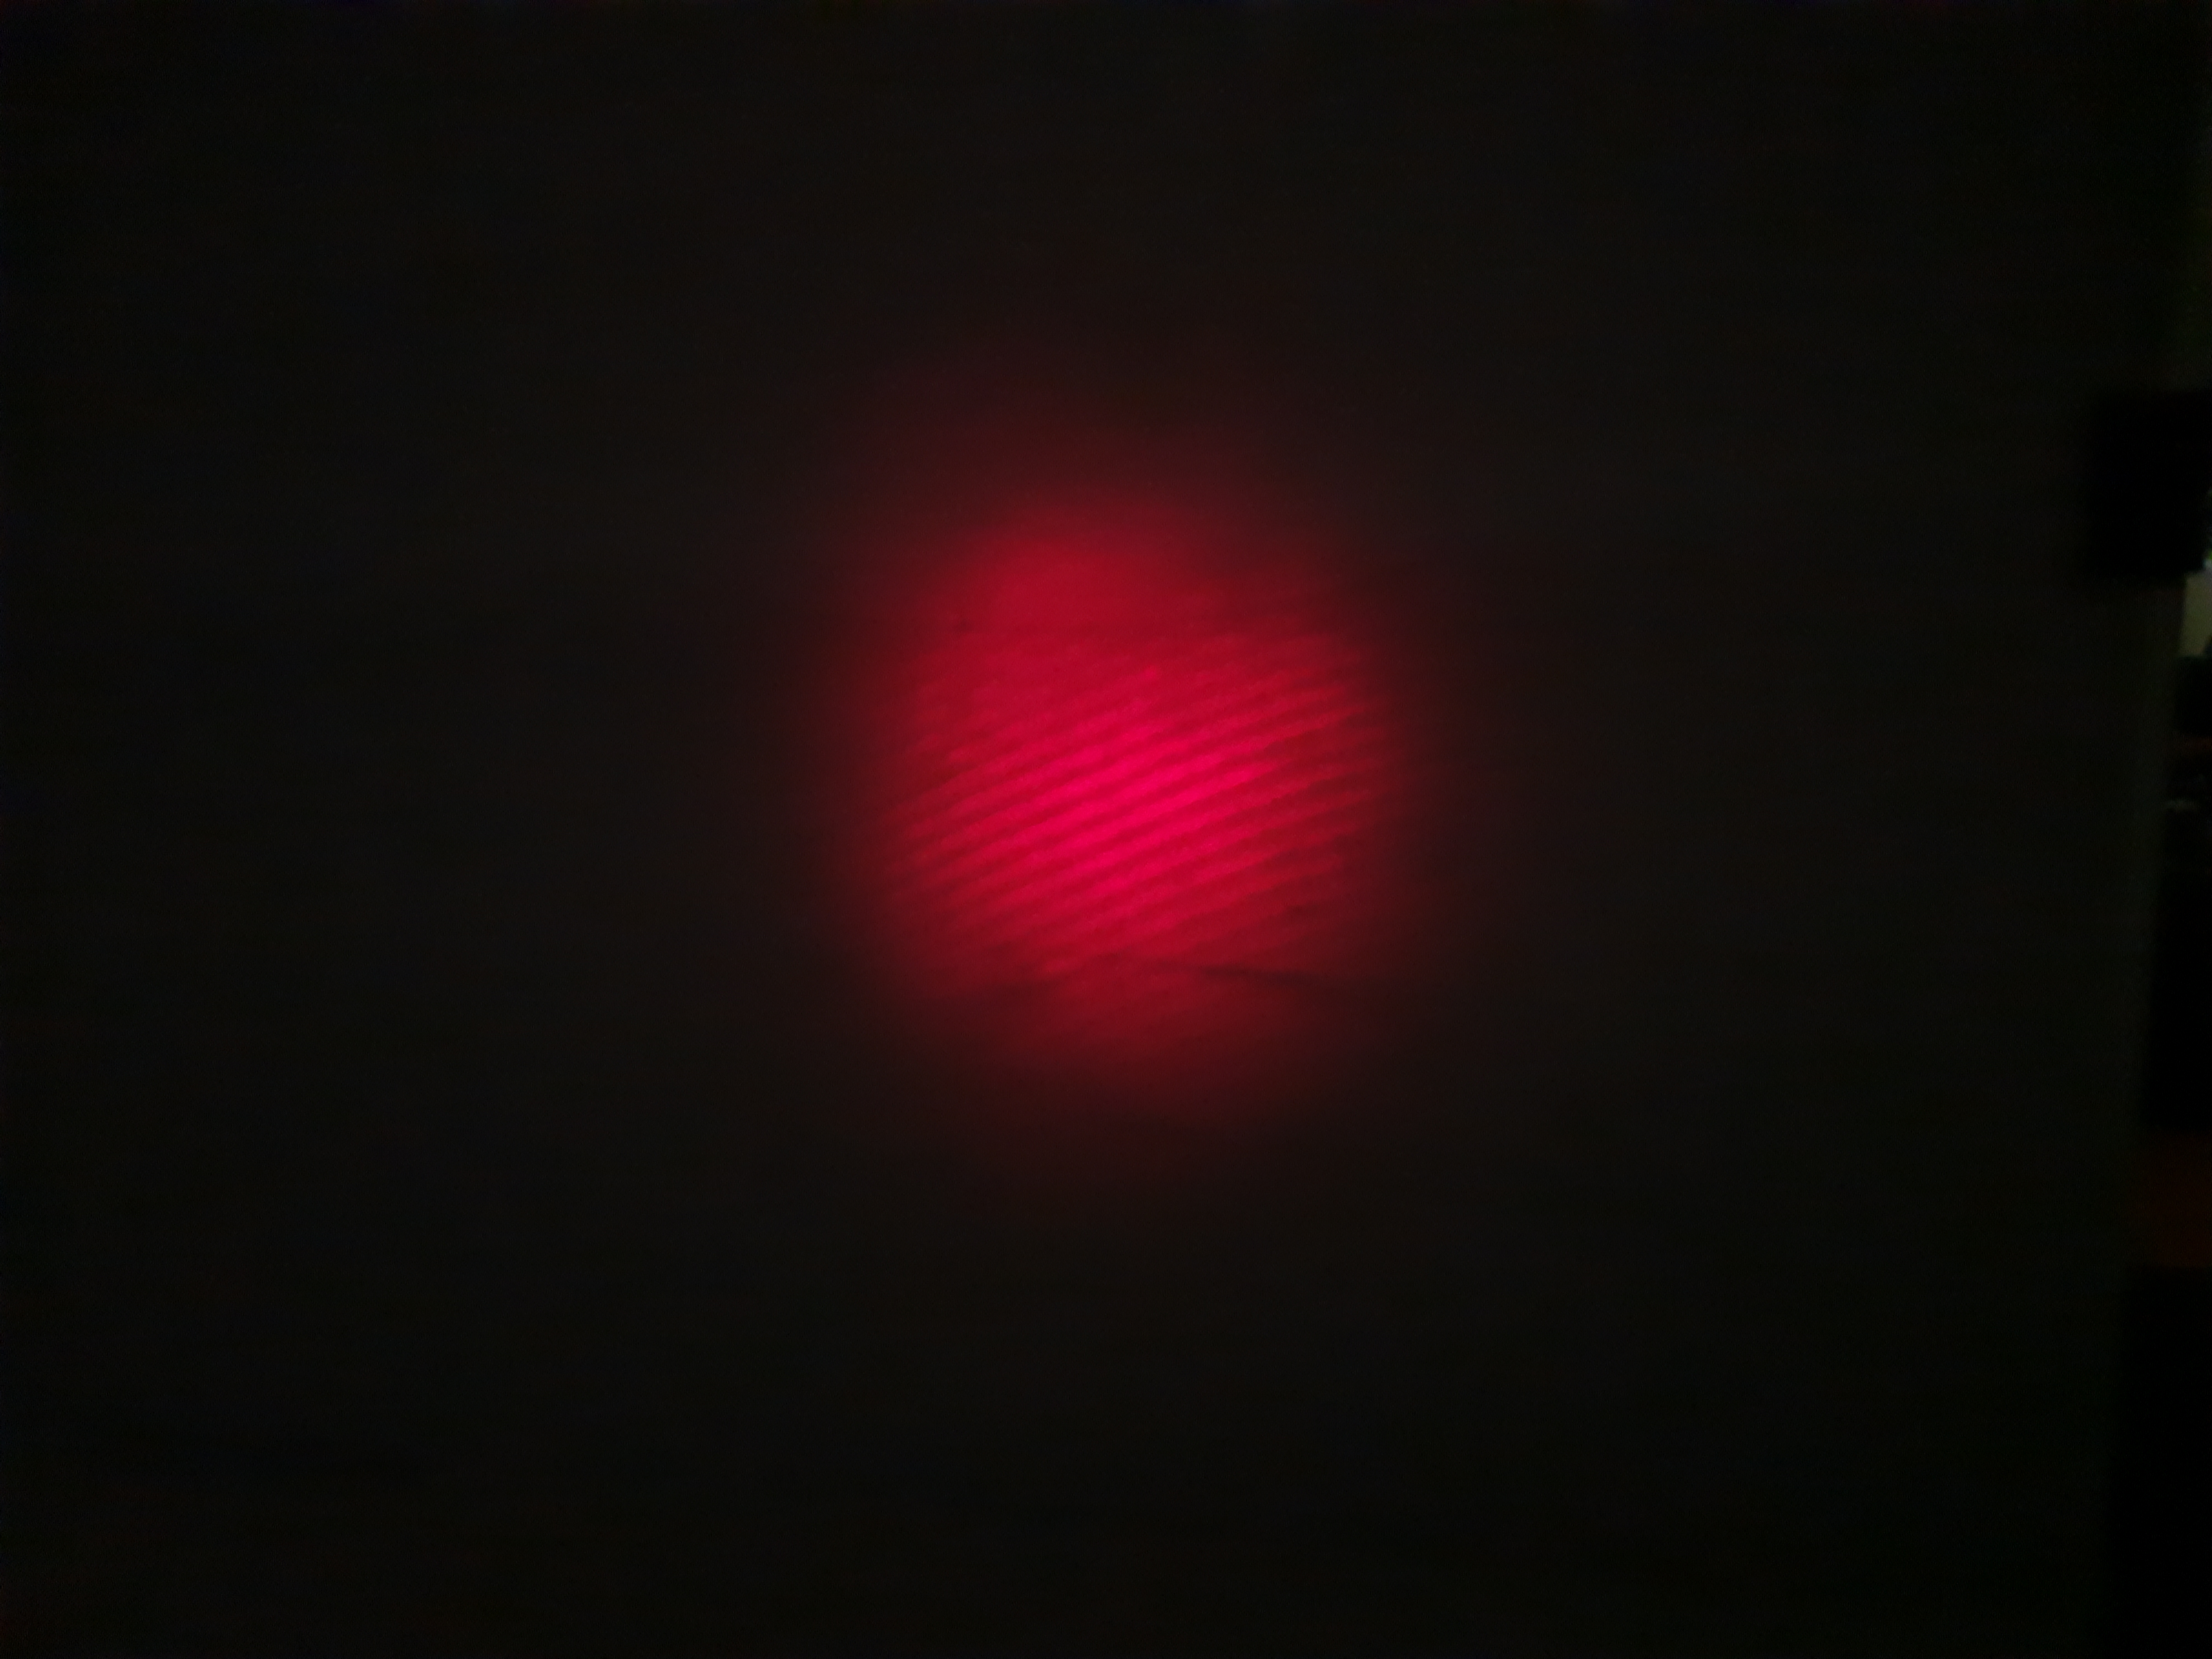
\includegraphics[width=8.3cm]{st} 
   \caption{Straight line fringes when mirrors are tilted by an angle $\theta$ intersect with each other}
   \label{st}
\end{figure}

The fringes of equal inclination is seen is shown in Figure (\ref{redf}). While the mirror moves in one direction, the fringes begin to disappear, there will be a point where two mirrors are equidistant from the beam splitter giving no fringes and then starts to appear. If you disturb the alignment of the mirrors with an angle $\theta$, fringes of equal thickness could be observed as shown in Figure (\ref{gd}). At the intersection of the mirrors, straight line fringes could be seen as shown in Figure (\ref{st}).

If the He-Ne Laser is replaced by sodium lamp, the fringes are seen in naked eye. It was observed that the fringes were of very low intense and was difficult to count the fringes. Therefore, only few readings was taken for that reason. It is certain that in this case the error in $\lambda$ will be large. The calculations and data analysis will be done in the following section. 

\pagebreak

\section{Analysis}
\begin{figure}[htbp] %  figure placement: here, top, bottom, or page
   \centering
   \includegraphics[width=8cm, height=14cm]{michelson.jpg} 
   \caption{Plot of $\Delta d$ versus N (a) for He-Ne Laser (b) for Sodium vapour lamp}
   \label{plot}
\end{figure}

From the Figure (\ref{plot}) (a) and (b), the slope ($\frac{\Delta d}{N}$) was found to be $0.00031778\pm0.00000460$ mm  and $0.00028349\pm0.00000861$ mm, by linear fit. Therefore, from equation (\ref{f}), the wavelength of light source $\lambda$ could be found by:
\begin{equation} \label{slop}
\lambda=2\times \text{Slope}
\end{equation}

Hence, from equation (\ref{slop}), the wavelength of He-Ne laser ($\lambda_{laser}$) turns out to be $635.56\pm9.20$ nm and wavelength of sodium lamp ($\lambda_{Na}$) turns out to be $566.98\pm17.22$ nm. $\lambda_{laser}$ lies within the literature value i.e 632.8 nm. $\lambda_{Na}$ has large error and doesn't lie within the range where literature value is 589.3 nm. The experimentally obtained value of $\lambda_{Na}$ corresponds to yellow light. This error in $\lambda$ is due to few number of readings taken for the sodium light as it was difficult to count the number of fringes disappearing / appearing. The instrumentation errors play important role in this experiment, as the intensity of the laser beam and sodium lamp was also low, there could be error in counting the number of fringes while moving the mirror. This could be improved by using the better quality glass plates with aligning the sodium light source in a beam. The random errors also come into picture as the experiments for two different cases were performed in two different days with varying temperature and humidity. It can be reduced by setting up the optimal temperature of the lab, around $20^{\circ}$C and using dehumidifier as it prevents the condensation on the surface of the mirrors and lenses and humidity damage to the laser source. 

\section{Conclusion}
From this experiment, we determined the wavelength of light, used to form fringes, by Michelson's interferometer. The He-Ne laser beam and sodium lamp was used. It was found that the wavelength of He-Ne laser ($\lambda_{laser}$) is 635.56 ± 9.20 nm and wavelength of sodium lamp ($\lambda_{Na}$) is 566.98 ± 17.22 nm. The $\lambda_{laser}$ closely agrees with the literature value 632.8 nm but there is a large error in case of $\lambda_{Na}$ due to random errors, human errors etc. 

The fringes of equal inclination is observed, when the virtual image of one mirror is parallel to other mirror and fringes of equal thickness is seen, when virtual image of one mirror is tilted to other mirror forming an air gap. There exists a point when both the mirrors coincide in both cases, where no fringes and straight line fringes are obtained respectively.

\section{Precautions}
\begin{enumerate}
\item{Turn the fine adjustment knob slowly in one direction to avoid backlash error.}
\item{Avoid eye exposure with the laser beams.}
\item{Use safety goggles when you begin the experiment.}
\item{Avoid touching the any reflecting surface of optics instruments with your fingers.}
\item{Before beginning the experiment use alcohol to clean the the surfaces of the surfaces.}
\item{Observing fringes through reflecting surface, in case of laser beam, is discouraged.}
\item{Maintain good temperature and control the humidity in the laboratory}
\end{enumerate}

\section{References}
\begin{enumerate}
\item{Ghatak, Ajoy (2009), Optics (4th ed.)}
\item{\url{https://www.niser.ac.in/sps/sites/default/files/basic_page/michelson%20interferometer.pdf}}
\end{enumerate}

\end{document}